\subsection{Introducción Twig}%
\label{sub:introducción_twig}

Twig es el motor de \textit{templates} por defecto de \textbf{Symfony}, permite reutilizar elementos de la vista en distintas partes de una aplicación web\@. Además, permite incluir lógica simple a la
vista de manera que sea fácil de comprender y entender\@. Un motor de \textit{templates} permite, entre otras cosas, reutilizar la estructura básica de una página y cambiar o sobrescribir
aquello que varía.

Twig funciona mediante el uso de \textbf{bloques}, los cuales son etiquetas que delimitan secciones del \textit{template}\@. Estas etiquetas tienen la función de indicarle al motor de \textit{templates}
que un \textit{template} \textit{hijo} puede sobrescribir estas partes del \textit{template}\@. De esta manera se consigue separar las partes estáticas del sitio, de aquellas que son dinámicas.


\subsection{Vista de Persona}
\label{sub:vista_persona}
Se creó una vista mediante la cual se pueda acceder a la información de cada persona y a la lista de actividades en las que se encuentra involucrada. Su
implementación se basó en la iteración de la colección de actividades  de la persona y la generación de html mediante \textbf{Twig}\@.
Como último paso se agregó estilo mediante \textbf{CSS} y una simple animación en \textbf{Javascript}.


\subsubsection{Estilo}%
\label{ssub:estilo}

Se utilizó una distribución de elementos utilizando \textit{grid}, una característica de \textbf{CSS} que permite acomodar elementos en una grilla\@. En primer lugar, se comenzó heredando de un template
general de \textbf{Sonata-Admin} denominado \textbf{standard\_layout} y se sobrescribió la sección o el bloque \textbf{sonata\_admin\_content}, que es la parte en la cual se muestra el contenido de cada
acción.



En un principio, se decidió por asignar los elementos de acuerdo a la figura~\ref{fig:image/grid}. Esto quiere decir que se separó el contenido en tres contenedores: el título, la lista de actividades y
los datos personales.


Dado que entre persona y actividad hay una relación de 1-n, cada \textit{objeto} \textbf{Persona} cuenta con una colección de actividades\@. Por lo tanto, se decidió definir un contenedor para cada una,
mediante la utilización de un bucle \textit{for} en \textbf{Twig}. Como resultado, se crea un contenedor y se inserta los datos por cada actividad presente en la colección\@. El resultado de esta
operación puede observarse en la figura~\ref{fig:image/vista_persona}\@.


Cada ítem de actividad está compuesto por un contenedor que actúa de \textit{header}, y otro que almacena los datos\@.




Se agregaron links en cada item de actividad, uno para visualizar la actividad y otro para modificarla, esto se logró obteniendo el nombre de la ruta desde una función en la entidad y generando
la ruta mediante la función
\textit{path} que provee \textbf{Twig}\@. Además, se agregó un link que permite, mediante \textbf{Javascript}, expandir o colapsar el contenedor de los datos de actividad\@. Estos links se agregaron en
el \textit{header} de cada actividad\@.

\subsubsection{Obtención de rutas}%
\label{ssub:obtención_de_rutas}
En \textbf{Symfony}, el nombre de una ruta actúa de identificador de la misma\@. Si se quiere generar una ruta, es necesario proveer como parámetro el nombre de la misma.


\textbf{Sonata} define sus rutas de la siguiente forma: \\

\textbf{admin\_app\_\{nombre\_de\_clase\}\_action} \\

Por ende, se optó por generar el nombre de la ruta a partir del nombre de la clase de la entidad. Esto quiere decir que, si se tiene una nombre de entidad igual a \textbf{Secretario}, mediante
operaciones de
manipulación de \textit{cadenas}, transformarla de \textbf{Secretario} a \textbf{admin\_app\_secretario\_acción}\@.



Para generar las rutas de edición o visualización de cada elemento, es necesario tener el nombre de la ruta en particular. Para lograr esto, se creó un método en cada entidad, que permite obtener el
nombre de la ruta, a través del nombre de la clase.






% TODO   franco continuar vie 01 nov 2019 20:37:16 -03

\begin{figure}[h]
    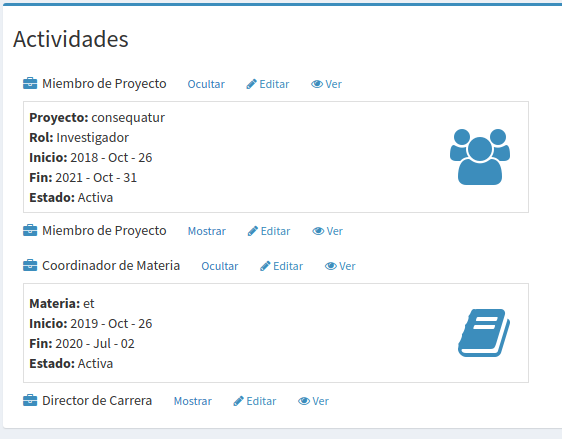
\includegraphics[width=1\linewidth]{image/vista_persona.png}
    \caption{Listado de actividades.\newline \textbf{Fuente:} Elaboración propia, captura de pantalla de aplicación web.}
    \label{fig:image/vista_persona}
\end{figure}


\begin{figure}[h]
    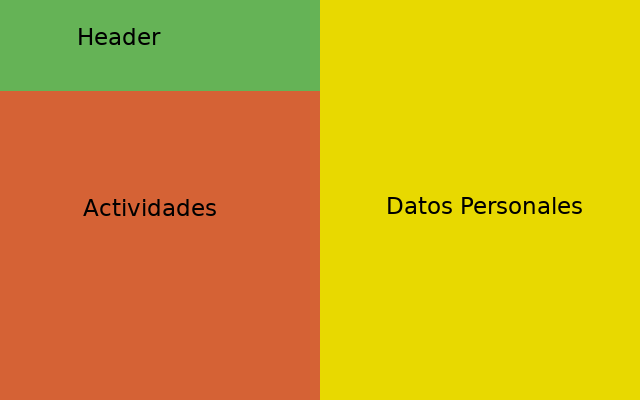
\includegraphics[width=1\linewidth]{image/grid.png}
    \caption{Distribución de columnas y filas.\newline \textbf{Fuente:} Elaboración propia.}
    \label{fig:image/grid}
\end{figure}
